\documentclass[runningheads]{llncs}
\usepackage{graphicx}
\usepackage[colorlinks]{hyperref}
\hypersetup{
    colorlinks = false,
    linkbordercolor = {blue}
}
\usepackage{listings}
\usepackage{courier}
\renewcommand{\floatpagefraction}{.8}
%
\begin{document}

\title{Augraphy: An Augmentation Pipeline API for Modern Document Images}
%\author{Alexander Groleau\inst{1,2} \and
%Kok Wei Chee\inst{1} \and
%Samay Maini\inst{1} \and
%Jonathan Boarman\inst{1}}
%
%\authorrunning{A. Groleau et al.}
%
%\institute{Sparkfish LLC (\email{augraphy@sparkfish.com})
%\and
%Left Associates LLC (\email{research@left.associates})}

\author{Anonymous ICDAR 2023 submission}

\maketitle

\begin{abstract}
We introduce Augraphy, a library for constructing feature augmentation pipelines for building modern document image datasets suitable for machine learning tasks. A discussion of prior art in the synthetic document image distortion space precedes description of the motivation for and structure of Augraphy. The library is used to quickly produce a derivative of the NoisyOffice dataset, on which a simple convolutional neural network is trained, which on some metrics outperforms the same network trained on the NoisyOffice set; the results of this experiment are discussed, followed by a look forward to further anticipated work.
\end{abstract}

\section{Introduction and Motivation}
Augraphy was created as a way to generate features that mimic those of real-world dirty documents, enabling users to produce datasets useful for training denoisers, layout classifiers, optical character recognizers, shadow and watermark removers, binarizers, deblurrers, defaders, layout classifiers, document image segmenters, and many other model types. Training supervised learning models requires labeled datasets, which contain pairs of training data objects and associated labels, or ground-truths. However, collecting or otherwise determining a set of labels for training data is quite challenging.  In the case of text documents, most real-world dirty documents /can't/ come with clean ground-truths.\\

Most often, source documents are too old, and often were created before the advent of digital storage media. Some documents are one-offs, produced ad-hoc in the typewriter era, but many more still were printed directly from the text editor used to write them, with no copy saved even after it became possible to do so. Document analysis and understanding tasks require these clean images for analysis. For these reasons, it's much easier to take clean documents and add distorting features to them with a tool like Augraphy than to start with the warped images and find or create ground-truths.

\section{NoisyOffice}
Many document-focused datasets exist, but most are designed for tasks like layout detection \cite{ref_RDCL2019}, content extraction \cite{ref_tobacco800}, or handwriting recognition \cite{ref_icdar}. the only publically-available dataset we could find that was exclusively focused on digitally-generated modern documents was NoisyOffice \cite{ref_NoisyOffice}.\\

This database \cite{ref_NoisyOfficeDatabase}, hosted on the UCI Machine Learning Repository \cite{ref_UCIMLR}, was created for training image processing filters, including denoisers and superresolution models. NoisyOffice includes three types of image:

\begin{enumerate}
\item ground truth images, created by printing some text and re-digitizing the physical document with a digital scanner,
\item synthetic noisy images, created by digitally fusing the text foreground with a background image of a coffee-stained or boot-printed page, using technique 1 above, and
\item real noisy images, created by physically stepping with boots onto physical documents, adding real coffee stains, and so on.
\end{enumerate}

Assembling the NoisyOffice database was a great service to the document analysis community, but for our purposes, the set is too limited:

\begin{itemize}
\item it contains only 3 font sizes (footnote, normal, large), 3 font types (typewriter, sans-serif, Roman), italicized and nonitalicized text, and 4 types of noise (folds, wrinkles, coffee stains, and footprints), for a total of 72 unique images.
\item the text is all English-language
\item the corpus has already been converted to grayscale, removing any choice about which desaturation algorithm to use
\item the image sizes provided are quite small (540x420), though double resolution images are also provided for use in training superresolution models.
\end{itemize}

Rather than providing a direct answer to these, Augraphy does not generate the initial document image input to a pipeline, instead taking the approach of providing the tools for building a suitable dataset for any document image analysis task while relying on users to supply the ground truth images.

\section{DocCreator}
In our investigations, the NoisyOffice database was the only preexisting dataset of images of modern documents with realistic distortions we could find; the situation is no better for document-specific feature augmentation tools, with only DocCreator \cite{ref_DocCreator} seeming to occupy that niche.\\

DocCreator contains character-set-level distortions, a mechanism for overlaying characters onto an arbitrary paper texture akin to merge technique \#1, and also includes an experimental tool for fusing the document image onto one of several 3D meshes to simulate physical alterations to the document like a crumpled and smoothed page.\\

While an interesting piece of software in its own right, DocCreator is geared towards historical documents like ancient manuscripts and scrolls, and so is unfortunately poorly-suited to generating realistic images of \textit{modern} documents. Worse, the software is a monolithic what-you-see-is-what-you-get editor, with all internals written in \texttt{C++}, making it unsuitable for use either in a semi-automated data augmentation pipeline or by the majority of researchers and industry practitioners who are much more familiar with Python-based tools and expect language-level integration.

\section{Document Distortion, Theory \& Technique}
Many approaches exist for adding features to an image, and many types of feature can be generated. The most common types of features added are Gaussian noise, blurring, geometric transformations like scaling, rotating, translating, and cropping, downsampling, font weighting, and so on.\\

These types of feature are certainly useful in general image analysis and understanding, but bear little relation to the types of features commonly found in real-world documents. A sheet of paper out in the world begins its life as wood pulp, bleached, drained, and pressed flat by a long series of rollers. These are cut to size and stacked, then bound in reams and sent out for sale and use. This is the last time the sheet is clean in its useful lifetime, and even at this point, manufacturing defects can lead to variations in the paper, even between two pages in the same ream. At the point of use, these pages are loaded into a printer where they are stamped or dusted in toner and burned with lasers or sprayed with ink. Any of these processes may alter the local texture or global topology of the sheet. The pages may receive handwritten marks at any point before or after printing, and may subsequently be folded, creased, crumpled, flattened, burned, stained, soaked, or generally be subject to any of a million other operations. Any secretary can describe hundreds of different document distortion features; any schoolteacher, thousands.\\

Augraphy's suite of augmentations was designed to faithfully reproduce this level of complexity in the document lifecycle. Every feature just listed has either a direct implementation already within the library or on the development roadmap, with more planned.\\

Some techniques exist for introducing these features into images of documents, including but not limited to the following:
\begin{enumerate}
\item Text can be generated independently of the paper texture, and can be overlaid onto the "paper" by a number of blending functions, allowing a variety of paper textures to be used. The NoisyOffice team did this.
\item Similarly, any markup features may be generated and overlaid by the same methods.
\item Documents can be digitized with a commercial scanner, or converted to a continuous analog signal and back with a fax machine.
\item The finished document image can be used as a texture and attached to a 3D mesh, then projected back to 2 dimensions to simulate physical deformation. DocCreator has a function to do this.
\end{enumerate}

Augraphy already has a story for the first three, with the fourth in planning.

\section{Augraphy}
We were unable to find any tools for producing training images of modern documents, in a way suitable for automated use. The Augraphy library is our attempt at filling this gap.\\

The library contains 18 unique transformations — augmentations, in Augraphy's parlance — which may be sequenced into a pipeline object which carries out the image manipulation. Users of the library can define directed acyclic graphs of images and their transformations via the AugraphyPipeline API, representing the passage of a document through real-world alterations.\\

Augraphy attempts to decompose the lifetime of features accumulating in a document by separating the pipeline into three phases: ink, paper, and post. The ink phase exists to sequence effects which specifically alter the printed ink — like bleedthrough from too much ink on page, extraneous lines or regions from a mechanically faulty printer, or fading over time — and transform them prior to "printing". The paper phase is concerned with transformations of the underlying paper on which the ink gets printed; here we find the PaperFactory generator for creating a random texture from a set of given texture images, as well as effects like random noise, shadowing, watermarking, and staining. After the ink and paper textures are computed separately, they are merged in the manner of Technique 1 from the previous section, simulating the printing of the document. After "printing", the document enters the post-phase, wherein it may undergo alterations that would affect an already-printed document out in the world. Augmentations are available here which simulate the printed page being folded along multiple axes, marked by handwriting or highlighter, faxed, photocopied, scanned, photographed, burned, stained, and so on. Figure 1 shows the individual phases of an example pipeline combining to produce a noised document image.
\begin{figure}
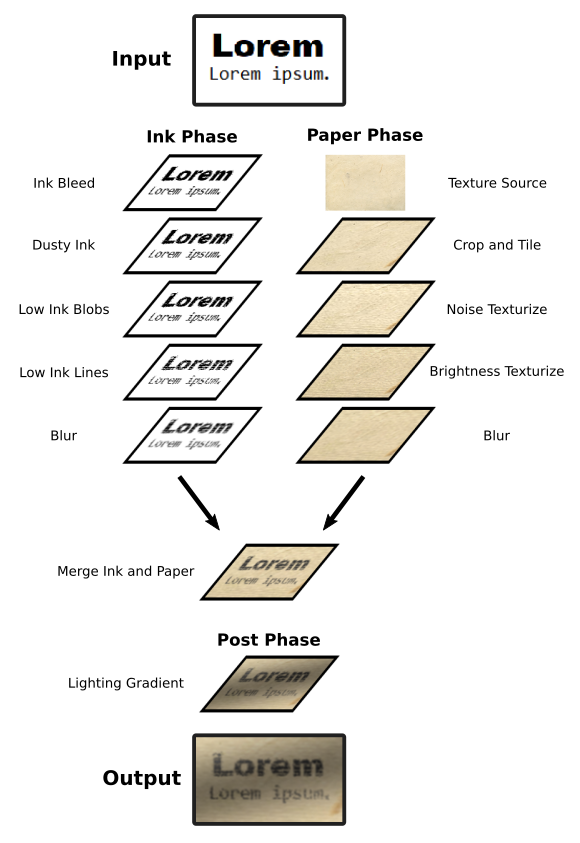
\includegraphics[width=\textwidth]{pipeline.png}
\caption{Visualization of an Augraphy pipeline.} \label{fig1}
\end{figure}

\section{The Augraphy API}
The library was developed in Python, to allow maximal accessibility for practitioners, and was designed with an object-oriented structure, with concerns divided across a class hierarchy. When composed, different parts of the library interact to produce complex sequences of document image transformations, generating new synthetically-augmented datasets.\\

Modern frameworks for machine learning like \texttt{fastai} \cite{ref_fastai} aim to simplify the data handling requirements, and concordantly, the Augraphy development team takes great pains to ensure our library's ease-of-use and compatibility. We wanted the library to be immediately useful with little effort, especially as part of a preprocessing step for training machine learning models, so great care was taken to establish good defaults. The default Augraphy pipeline makes use of all of the augmentations available in Augraphy, with starting parameters selected after manual visual inspection of several thousand images. Adding a diverse array of realistic features to documents can be done with the following five-line incantation:
\begin{lstlisting}[language=Python]
from augraphy import *
pipeline = default_augraphy_pipeline()
img = cv2.imread("image.png")
data = pipeline.augment(img)
augmented_img = data["output"]
\end{lstlisting}

\subsection{Base}
\texttt{augraphy.base} is the core of the library, containing the central class for augmentations, another class for sequences of augmentations, and the pipeline class itself. The base classes exist to coordinate the compilation of discrete transformations into a larger pipeline, and to facilitate the operation and maintenance of these.\\

There are four ''main sequence'' classes in \texttt{augraphy.base}, which together provide the bulk of the library's functionality. Two additional classes, \texttt{OneOf} and \texttt{PaperFactory}, provide additional variation to pipelines in ways explored soon.

\subsubsection{Augmentation}
Augmentation is the most basic class in the project, and essentially exists as a thin wrapper over a probability value in the interval [0,1]. Every augmentation object is constructed with a probability of that augmentation being applied during the execution of a pipeline containing it.\\

This class also contains a method which interacts with the probability data, dynamically generating a second floating point probability value and using this to decide whether the augmentation should be applied at runtime.

\subsubsection{AugmentationResult}
After an augmentation is applied, the output of its execution is stored in an \texttt{AugmentationResult} object and passed forward through the pipeline. These objects also record an exact copy of the augmentation object that was instantiated and applied, as well as any metadata that might be relevant for debugging or other advanced use.

\subsubsection{AugmentationSequence}
A list of \texttt{Augmentation}s -- together with the intent to apply those Augmentations in sequence -- determines an \texttt{AugmentationSequence}, which is itself both an \texttt{Augmentation} and callable. In practice, these are the model for the pipeline phases discussed previously; they are essentially lists of \texttt{Augmentation} constructor calls which produce callable \texttt{Augmentation} objects of the various flavors explored in . \texttt{AugmentationSequences} are applied to the image during each of the \texttt{AugmentationPipeline} phases, and in each case yield the image, transformed by some of the Augmentations in the sequence.

\subsubsection{AugmentationPipeline}
The bulk of the innovation in Augraphy resides in the Augmentation pipeline, which is an abstraction over one or more events in a physical document's life. Events in this case could be the initial printing of the document when ink adhered to the paper material, or several weeks later when the document was adhered to a public board, annotated, defaced, and torn away from its securing staples. Fifty years later, our protagonist page resurfaces in the library archive during routine preservation-scanning efforts. Conservationists use delicate tools to gently position and record an image of the document, storing this in a public repository. An \texttt{AugmentationPipeline} can model this entire sequence of events, or any individual event within.\\

Realistically reproducing effects in document images requires rethinking how those effects are produced in the real world. Many issues, like the various forms of misprint, only affect text and images on the page. Others, like a coffee spill, change properties of the paper itself. Further still, there are transformations like physical deformations which alter the geometry and topology of both the page material and the graphical artifacts on it.\\

Effectively capturing processes like these in reproducible augmentations meant separating our model of a document augmentation pipeline into ink, paper, and post-processing layers, each containing some augmentations that modify the document image as it passes through. Augraphy pipelines, then, are constructed from three sequences of augmentations, to be applied one after the other in each of those phases. After transformations occur to the ink and to the paper separately, the pipeline fuses them together, simulating the printing of that ink on that paper. Changes to the document after that point happen within the post layer, where we might find effects like crumpling up the page and smoothing it out again, or using a pen to underline a section of text.\\

Use of the Augraphy library to produce a dataset for model training — will be covered in some detail later — boils down to the definition and application of one or more pipelines to one or more images.\\

The value added by the \texttt{AugrapyPipeline} class over a bare list of functions mapped over an image is principally in the collection of metadata: the output of an \texttt{AugraphyPipeline} application is a Python dictionary which contains not only the final image, but copies of every intermediate image, as well as information about the object constructors and their parameters that were used for each augmentation. This allows for easy inspection and fine-tuning of the pipeline definition to achieve outputs with desired features.

\subsubsection{OneOf}
Real-world processes generally allow for objects to exist in multiple states over time. To model the possibility that a document image has undergone one and only one of a collection of augmentations, we use \texttt{OneOf}, which simply selects one of those augmentations from a given list, and uses this to modify the image.

\subsubsection{PaperFactory}
We often print on multiple sizes and kinds of paper, and out in the world we certainly \textit{encounter} such diverse documents. We introduce this variation into the \texttt{AugmentationPipeline} by including \texttt{PaperFactory} in the \texttt{paper} phase of the pipeline. This augmentation checks a local directory for images of paper to crop, scale, and use as a background for the document image. The pipeline contains edge detection logic for lifting only text and other foreground objects from a clean image, greatly simplifying the "printing" onto another "sheet", and capturing in a reproducible way the construction method used to generate the NoisyOffice database. Taken together, \texttt{PaperFactory} makes it effectively possible to re-print a document onto other surfaces, like hemp paper, cardboard, or wood.

\subsection{Augmentations}
The \texttt{base} modules provide scaffolding for working with general transformations on document images, called \texttt{augmentations}. We have already included many such transforms in the standard library, and have also provided utilities for easily building new augmentations and integrating them into the Augraphy workflow.\\

Augraphy was designed to replicate effects seen in real-world documents in training data for image models, so each augmentation represents a feature that will appear in the final dataset. Augmentations come in many flavors and types, varying not only in their visual effect but also in their software design. Other libraries already exist for adding basic effects like blur, scaling, and rotation; Augraphy includes augmentations for these as well. The more interesting effects come from a combination of primitive effects, and mimic document types out in the world.\\

Figures 2 and 3 contain representative images of each augmentation applied to this very document. Descriptions of and motivation for each augmentation are available on GitHub \footnote{\url{https://github.com/sparkfish/augraphy}}.

\begin{figure}
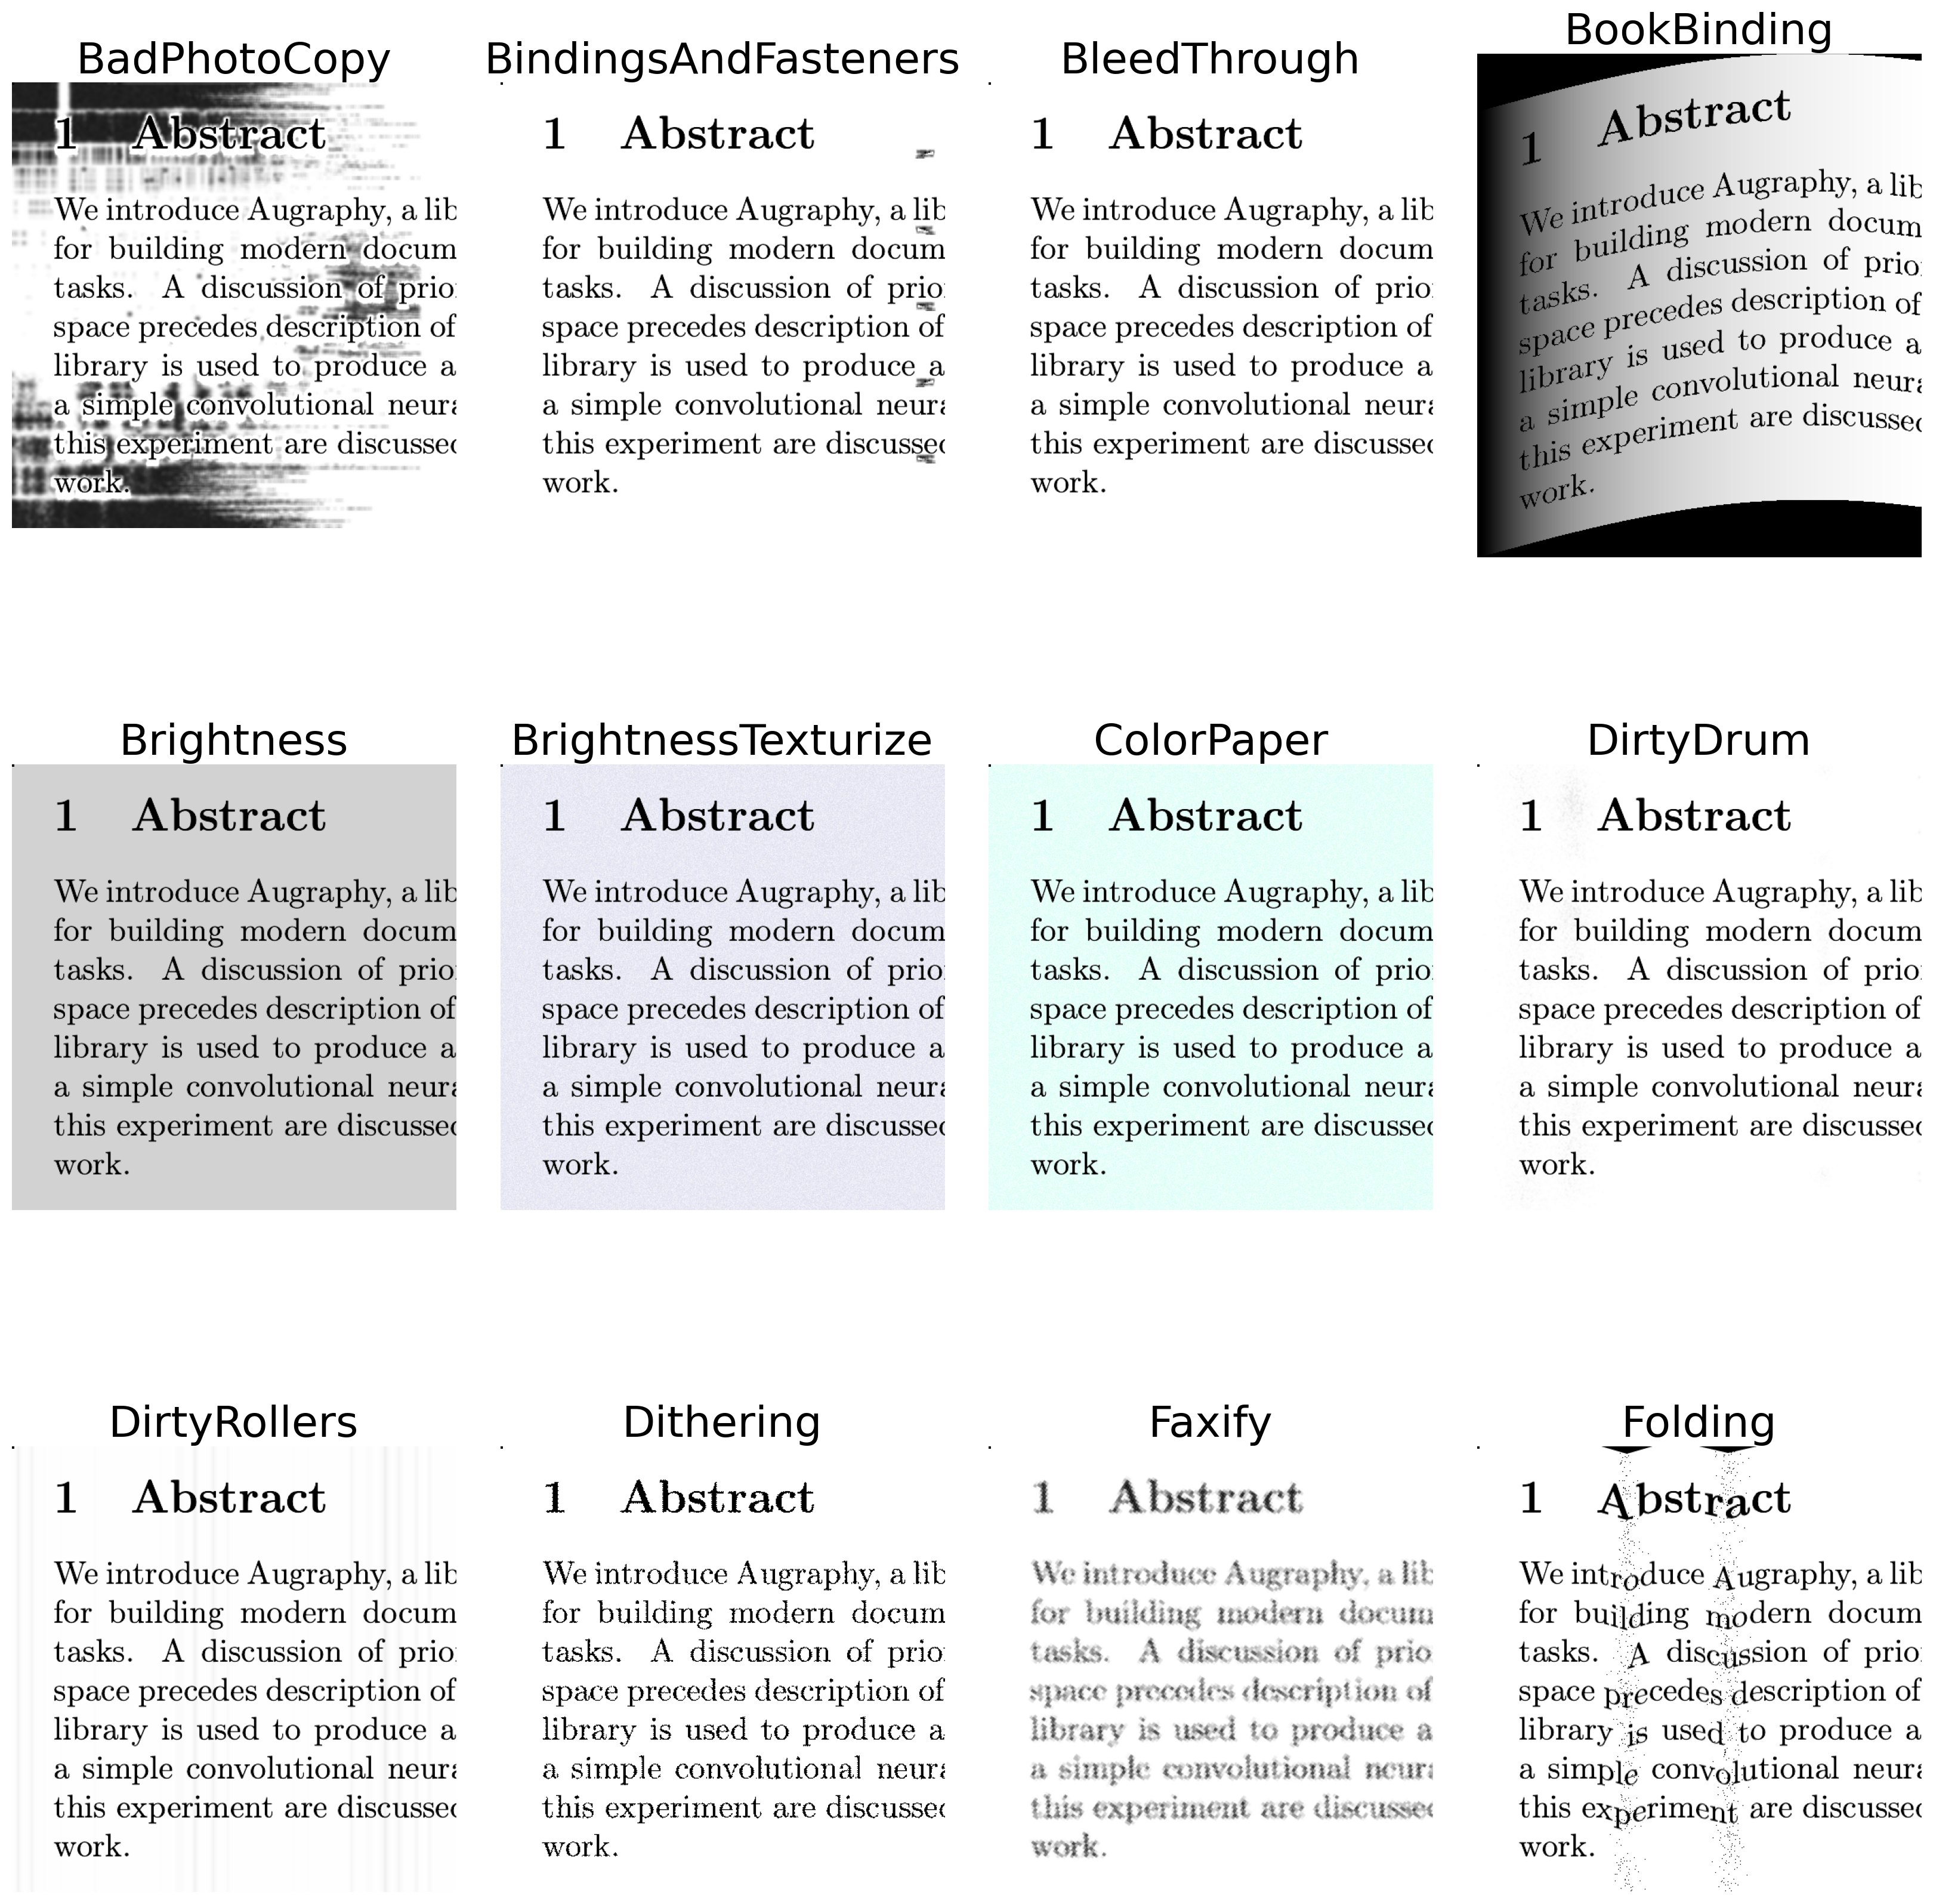
\includegraphics[width=\textwidth]{augmentations1.png}
\caption{Examples of each augmentation.} \label{fig2}
\end{figure}

\begin{figure}
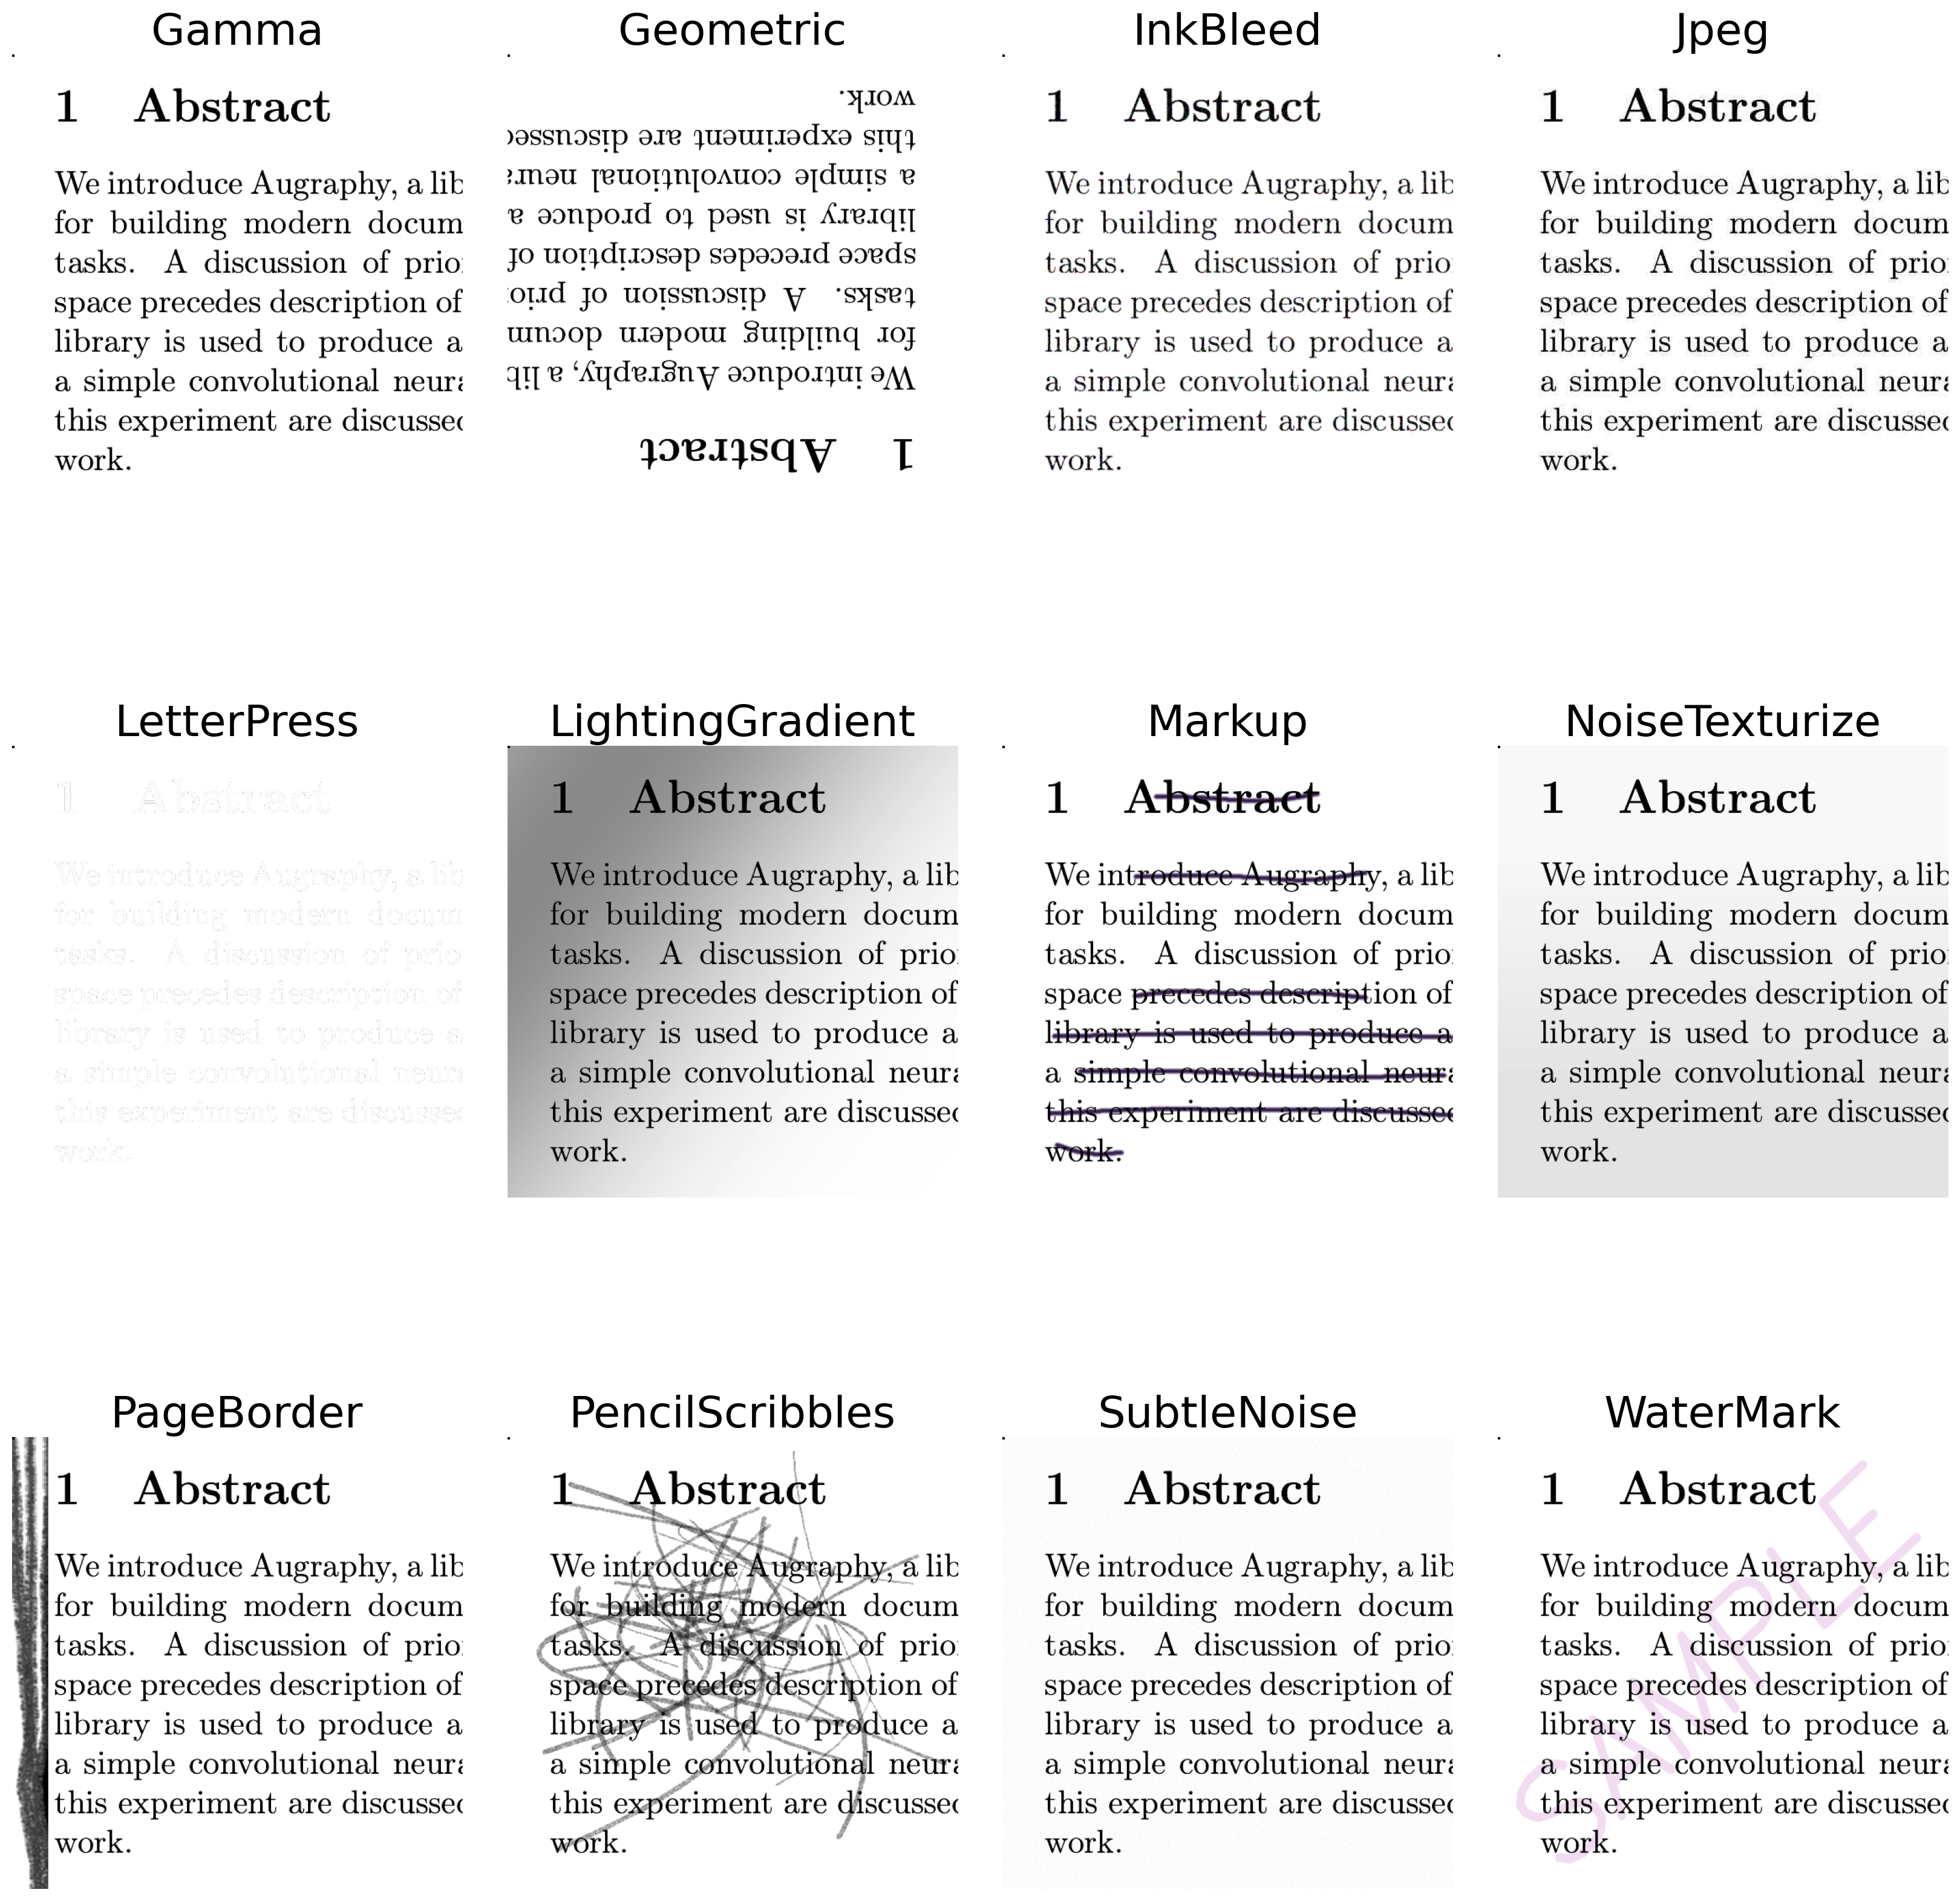
\includegraphics[width=\textwidth]{augmentations2.png}
\caption{Examples of each augmentation.} \label{fig3}
\end{figure}

\subsection{Utilities}\label{utilities}
Interoperability and flexibility are core requirements of any data augmentation library, so Augraphy includes several utility classes designed to improve developer experience. Chief among these are \texttt{ComposePipelines}, \texttt{Foreign}, and \texttt{ImageOverlay}, which respectively

\begin{enumerate}
\item provide a means of composing two pipelines into one, allowing for the construction of complex pipeline algebras,
\item wrap augmentations from projects like \texttt{Albumentations} \cite{ref_albumentations} and \texttt{imgaug} \cite{ref_imgaug}, and
\item uses various blending algorithms to fuse foreground and background images together, useful for simulating "printing".
\end{enumerate}
\section{Deep Learning with Augraphy}
Augraphy aims to facilitate rapid dataset creation, advancing the state of the art for document image analysis tasks. This section describes a brief experiment using Augraphy to augment the NoisyOffice set, producing a corpus that is used to train a denoising convolutional neural network which outperforms an identically-structured model trained on only the provided NoisyOffice data. We continue to return to this database when testing our model training pipelines and new architectures, and felt it an appropriate jumping-off point for Augraphy analysis.

\subsection{Model Architecture}
To evaluate Augraphy, we trained a U-net convolutional neural network, built with the Keras library. This network achieved a high score on the NoisyOffice Kaggle competition \footnote{\url{https://www.kaggle.com/code/michalbrezk/denoise-images-using-autoencoders-tf-keras/notebook}}; we selected this one for its simplicity and the clarity of its exposition, and use it with few changes.\\

This low-layer model contains two layers of a convolution, each followed by a rectified linear unit activation function, then a batch normalization layer as the encoding step. After the encoding step, max pooling is applied, followed by dropout, to improve translation invariance of feature encoding and to avoid overfitting respectively. The decoding step closely mirrors the encoding step, and contains two layers of ReLU-activated convolutions followed by a batch normalization layer, but with the convolution dimensions reversed; in this case the model is "unpacking" higher-dimensional features from its low-dimensional latent representation. After the decoding step, we perform 2-dimensional upsampling, compensating for the 2D max pooling applied earlier. Finally, the output of previous layers is convolved with a 3x3 kernel, while retaining the same image dimensions. This final convolution uses the sigmoid function as its activation function. All convolution steps use a 3x3 kernel and pad edges with zeroes, the max pooling and upsampling steps both use 2x2 kernels, and a 50\% unit dropout rate was used.

\subsection{Data Generation}
Despite recent techniques [Training Vision Transformers with Only 2040 Images, Vision Transformer for Small-Size Datasets, Training a Vision Transformer from scratch in less than 24 hours with 1 GPU] for reducing the volume of input data required to train models, data remains king; feeding a model more data during training can help ensure better latent representations of more features, improving robustness of the model and increasing its ability to generalize.\\

The NoisyOffice data provided by Kaggle contains 144 ground truth images, 144 training images, and 72 validation images. For the Augraphy model, we produced a dataset 10x larger, by duplicating each of the ground truth images, then running 10 Augraphy pipelines against each copy. Doing this was trivial; Augraphy's value lies in its ease of use in producing large training sets.\\

The NoisyOffice dataset contains folded sheets, wrinkled sheets, coffee stains, and footprint noise. The features given by the wrinkle and fold distortions can be mimicked by overlaying the foreground text on wrinkled and folded paper textures, as the NoisyOffice team did, and the features created by the stains and footprints can be mimicked by introducing dark regions and thin lines. With Augraphy, we expected that we could use the BadPhotoCopy augmentation to produce the dark regions and a combination of the strikethrough behavior from the Markup augmentation and the smooth curve shading behavior of the PencilScribbles augmentation to add the last feature to the ground-truth data. The PaperFactory augmentation makes the paper texture overlay trivial and repeatable. In the end, we executed the following pipeline:

\begin{lstlisting}
ink_phase = []
paper_phase = [PaperFactory(p=0.5)]
post_phase = [
  BadPhotoCopy(p=0.5),
  PencilScribbles(p=0.5),
  Markup(markup_color=(0,0,0), p=0.5)
]

AugraphyPipeline(ink_phase, paper_phase, post_phase)
\end{lstlisting}

In each of the augmentations created above, the probability of applying to the image passing through the pipeline was set to 50\%, and the strikethrough behavior (the default) for the Markup augmentation was set to strike out words with only black lines.\\

The PaperFactory augmentation reads and randomly crops image textures from a local directory; to this we added two \footnote{\url{https://p2.piqsels.com/preview/642/889/110/paper-crease-creased-texture.jpg
}}, \footnote{\url{https://blog.miklavcic.si/wp-content/uploads/2011/11/white_paper_1.png}} public domain images of wrinkled paper found on Bing.

\subsection{Training Regime}
We fit the model architecture described in the previous section to both the NoisyOffice corpus and a derivative work generated with Augraphy applied to the NoisyOffice ground truth images.\\

Training proceeded for 600 epochs or until the model began to overfit, with an overfit patience of 30 epochs. The NoisyOffice model finished training after 416 epochs, while the Augraphy model trained for the full 600 epochs.\\

Both models were trained with mean squared error as the loss function, using the Adam optimizer, and evaluated with the mean average error metric.

\subsection{Results}
Sample predictions from each model on the validation task are presented in Figure 1. As expected, the NoisyOffice model performs admirably, but does struggle to fully remove the coffee stain feature, leaving some residue. The Augraphy model clearly outperforms the NoisyOffice model at stain removal, but does not generalize well to the folding and wrinkling noise; this was expected, since the Augraphy training data did not include fold or wrinkle features. Further, the Augraphy model overcompensates for the \texttt{BadPhotoCopy} behavior on text, by increasing the line thickness in the predicted text, resulting in a bold font.\\

\begin{figure}\label{fig4}
\includegraphics[width=\textwidth]{sidebyside.png}
\caption{Validation images (left), with the images predicted by the NoisyOffice (center) and Augraphy (right) models.} \label{fig4}
\end{figure}

To compare the models' performance on the validation task, we considered the following metrics:
\begin{enumerate}
\item Root mean square error (RMSE)
\item Structural similarity index (SSIM)
\item Peak signal-to-noise ratio (PSNR)
\end{enumerate}

Over the last 5 epochs of training, the performance of the models on average loss, average mean-average-error (MAE), average validation loss, and average validation MAE were recorded. The models predicted cleaned versions of the validation images (Figure 4), which were then compared to the groundtruth versions according to each metric. The average over all such results obtained during validation was taken. These metrics are displayed in Table 1.

\begin{table}
\centering
\caption{Model training statistics and performance on NoisyOffice validation task}\label{tab1}
\begin{tabular}{|@{\hspace{2em}}l@{\qquad}|@{\hspace{2em}}l@{\qquad}|@{\hspace{2em}}l@{\qquad}|}
\hline
Metric & NoisyOffice & Augraphy\\
\hline
PSNR & 63.09152246942623 & 63.3491691640664\\
SSIM & 0.8726093605602885 & 0.8662918306486613\\
RMSE & 0.1878745854176291 & 0.18310202817380003\\
Test Loss & 0.0011 & 0.0012\\
Test MAE & 0.0150 & 0.0129\\
Validation Loss & 7.5551e-04 & 8.22202e-04\\
Validation MAE & 0.01236 & 0.01076\\
Training Time & 190ms/step & 218ms/step\\
\hline
\end{tabular}
\end{table}

The Augraphy model outperforms the PSNR score of the NoisyOffice model on the validation task by half a percent, and has a lower mean average error both in test and validation during training, but underperforms by 0.8\% on structural similarity and 2.5\% on RMSE in validation, with a higher average test and validation loss. These numbers are consistent with the visual prediction results displayed in Figure 1: the Augraphy model predicts fewer pixels in the text (RMSE lower by 2.5\%), but removes more noise and with a higher degree of fidelity than the NoisyOffice model (PSNR higher by 0.2576466946). The training metrics collected indicate that the Augraphy model has lower variance so is more precise than the NoisyOffice model, but exhibits higher loss and thus less accuracy in its predictions.

\section{Future Work}
This section describes new directions for research and development.

\subsection{Tuning the Pipeline}
The pipeline used to generate training data for the Augraphy model was extremely naive, and only contained four augmentations, most with default parameters, demonstrating Augraphy's high degree of both utility and ease-of-use. However, much of the data used in training contained an excessive amount of added noise, making the image unreadable to the human eye, and too noisy to recover text features from. Producing the most accurate model with Augraphy requires careful fine-tuning of the augmentation input parameters to generate training images closer to the validation set.

\subsection{Additional Techniques}
For brevity, this article only includes experimental results for one type of model. We plan to evaluate denoisers built with other architectures, particularly transformers, diffusion and generative adversarial networks, and ensembles of these. During the validation task, the naive Augraphy model correctly removed the page fold and wrinkle noise, but visually degraded regions of the foreground text. By comparison, the NoisyOffice model left more of the text intact, but permitted more of the stain features to remain in the output. Better results may be achieved by a sequential model built from an Augraphy-trained denoiser followed by an inpainting model to repair the text.\\

\subsection{An Augraphy Dataset}
Privacy and security concerns typically preclude the assembly of large sets of modern document images: most documents are not intended for general viewing. The authors have searched frequently, for over a year, and have been unable to find decently-sized (>10 images) sets of modern document images, besides the NoisyOffice set. We intend to release an Augraphy-generated dataset in the coming months.

\subsection{Augraphy Enhancements}
Several upgrades to the Augraphy library itself are also planned.

\subsubsection{Scaling}
While much work has gone into tuning Augraphy's defaults, and we feel that the effects produced are quite realistic, none of the augmentations were designed to be scale-invariant, and so we plan to introduce pre-trained networks into the library to generate effects in the future.

\subsubsection{Performance}
The authors typically run substantial Augraphy jobs on enthusiast or datacenter hardware. Performance enhancements to the library are already underway, which will decrease pipeline execution time dramatically, enabling faster creation of larger datasets on more common hardware.

\section{Conclusion}
We presented Augraphy, an augmentation framework for generating realistic datasets of modern document images. Two other players in the same space were examined and found lacking for our purposes, motivating the creation of this library. We described creating an Augraphy-noised version of the NoisyOffice dataset, then compared some preliminary results obtained by training a convolutional U-Net on these datasets. Finally, we discussed some future directions for research, and the continued evolution of this tool. Augraphy is licensed under the MIT open source license, and readers are invited to participate in its development on GitHub.


%
% ---- Bibliography ----
%
% BibTeX users should specify bibliography style 'splncs04'.
% References will then be sorted and formatted in the correct style.
%
\bibliographystyle{splncs04}
\bibliography{paper}

\end{document}

